\subsection{Adaptation of Fukuda's algorithm for polyhedra}

Is this section, Fukuda's algorithm is adapted for the vertex enumeration of unbounded polyhedra. For a given $H$-polyhedron, described by half-spaces, the objective is to find a set of vertices $V$ and a set of vectors $C$ such that $P = conv(V)+cone(C)$. Note that if a line directed by a vector $l$ is included in $P$, $\{l,-l\}\subset C$. 

\subsubsection{Converting to positive coordinates and detecting the linealy space}

Knowing a vertex of a polyhedron allows to find an affine transformation which sends it in the positive orthant. The process is to map the vertex to the origin and the normals of the hyperplanes defining it to the canonical base by respectively a translation and a change of basis.

Finding a vertex of the polyhedron is done using a dictionary as presented in Section~\ref{section_altsimplex}. In fact, obtaining a cobasis composed only by slack variables pushed to their bounds with all the other variables in their bounds gives a dictionary that describes a vertex of the polyhedron. Here the row corresponding to the cost function and the column corresponding to the constants are not used.


To do so, the first thing is to create a dictionary and to reach the feasible area, to check for emptiness. This is exactly the first phase of the simplex algorithm. Then, since the cobasis has to be composed only by slack variables, all the original variables in the cobasis are pivoted with a suitable slack variable (the corresponding coefficient has to be non null) but the assignments are not changed: it could bring the dictionary out of the polyhedron. 

\paragraph*{Detection of the linealty space:} The linealty space is the biggest affine subspace included in the polyhedron. If an original variable has no suitable slack variable to be exchanged with, it means this variable has no influence on the distance to each constraints, there is a line included in the polyhedron: an affine subspace has been found. To overcome this problem, two constraints are added with opposed normal vectors, their directions being the affine subspace's one, and the constant is zero for both. This provides a suitable slack variable to pivot around and the linealty space is saved, Example~\ref{ex_detect_linalty} illustrate this procedure. A cobasis full of slack variables means there exists enough independent constraints to define a vertex, and there is no linealty space exists. Since this phase adds new constraints, the feasible area might have to be reached again.

\begin{example} 
\begin{multicols}{2}
Let $-1\leq x+y\leq 1$ be two constraints, the corresponding dictionary is:
\begin{tabular}{| c | c || c c |}
\hline	
$x$ & $y$ & & \\
\hline
\hline	
$-1$ & $-1$ & = & $s_1$\\ \hline	
$-1$ & $-1$ & = & $s_2$\\ \hline 
\end{tabular}. $x$ can be pivoted with $s_1$:
\begin{tabular}{| c | c || c c |}
\hline	
$s_1$ & $y$ & & \\
\hline
\hline	
$-1$ & $-1$ & = & $x$\\ \hline	
$1$ & $0$ & = & $s_2$\\ \hline 
\end{tabular}. In this dictionary, $y$ and $s_2$ are independents, a pivot can't occur. It means that for all values of $y$ there is a suitable $x$ in the feasible area: there is and affine space directed by $(-1,1)$ included in the polyhedron. the constraints $-x+y=0$ are added.

\columnbreak

\figurecol{
\includegraphics[width=0.6\columnwidth]{images/linealty.eps}%
\figcaption{Geometrical interpretation of the constraints, with the feasible area shaded. The constraints represented with their normal vectors are added after detection of the linealty space}}
\end{multicols}
\label{ex_detect_linalty}
\end{example}

The last thing is pushing one by one the variables of the cobasis to their bounds. If doing so would make other variables violate their bounds, the variable is exchanged with the one which bound would be violated first, the latter is then set to its bound (note that the original variables have no bounds). A vertex is found with the hyperplanes that define it.

\paragraph{Complexity:} required to apply Fukuda's algorithm, this phase costs the finding of the feasible area, which is equivalent to a linear optimization, then pushing every variable to their bounds (which might imply pivoting for every variable). The final cost is $O(max(n,d)d^2+L(d,n))$ for a problem with $n$ half-spaces, $d$ dimensions and $L(d,n)$ the complexity of a linear optimization in $d$ dimensions and $n$ constraints. This can be neglected in front of the cost of Fukuda's Algorithm.

\subsubsection{Cone detection in Fukuda's algorithm}

Here the problem is reduced to the vertex enumeration of a potentially unbounded polyhedron in the positive orthant. Fukuda's algorithm allows to explore all the vertices. The unboundedness in general has no influence on the behaviour of the algorithm: it corresponds to a lack of constraints, while the algorithm just switches between the constrains.

The research of the cone relies on the following proposition:
\begin{proposition}
Let $P$ be a polyhedron. If $d$ hyperplanes intersect in a vertex $v$, and $d-1$ of them intersect in a line directed by a vector $l$, if $\forall k\in \mathbb{R}_+$, $v+kl\in P$, then $l$ belongs to the cone of $P$. The cone of $P$ is generated by the vectors obtained this way.
\label{prop_cone}
\end{proposition}

The belonging to the cone comes from it definition: the cone is the set of all the unbounded directions of the polyhedron. Let $V$ be the set $P$'s vertices and $L$ the set of vectors given by the proposition, the rest of the property is obtained by showing $P=conv(V)+cone(L)$. $conv(V)+cone(L)\subset P$ is already done, the other inclusion is obtained by, for any point of $P$, projecting with the vectors of $L$ until a bounded face is reached (all the point of a bounded face belongs to the convex hull of the vertices of the face).

Proposition~\ref{prop_cone} states that to find all the vectors of the cone, it is sufficient to check every vertex for the existence of a conic direction, i.e. directions such that $d-1$ independent constraints are saturated. Fukuda's algorithm explores the polyhedron and finds all the possible arrangement of constraints that defines the vertices, thus for every definition of a vertex, the dictionary is check for the existence of a cobasic variable that can be increased while not decreasing any other (not getting closer from an other constraint) and which decreases the objective function (not getting closer from an axis). Conversely, a vector found this way is a ray included in the polyhedron: it belong to the cone. The rays can be output several times, a suppression of the duplicates is done. Example~\ref{ex_detec_cone} illustrates the detection of a ray for a given dictionary.

\begin{example}
\begin{multicols}{2}	
	Cone detection with the dictionary:
	\begin{tabular}{| c | c || c || c c |}
	\hline	
	$x$ & $y$ & const & & \\
	$\downarrow$ & $\downarrow$ &$\downarrow$  & & \\
	\hline
	\hline		
   	$-1$ & $1$ & $2$ & = & $s_1$\\ \hline \hline	
   	$-1$ & $-1$ & $0$ & $\leftarrow$ & obj  \\
   	\hline
   	\end{tabular}. This dictionary corresponds to the constraints $x-y\leq 2$. As $s_1$ would be decreasing, $x$ does not provides a cone direction, yet $y$ does: the objective is decreased and $s_1$ increases: $(0,1)$ belongs to the cone.\\

\columnbreak

\figurecol{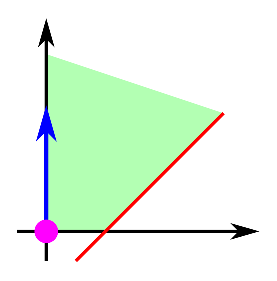
\includegraphics[width=0.6\columnwidth]{images/cone2.eps}%
\figcaption{Geometrical interpretation, the arrow represents the conic direction found.}}
\end{multicols}
\label{ex_detec_cone}
\end{example}

\paragraph{Complexity:} for each vertex, the existence of a conic direction is to be tested. This adds $O(gnd)$ to the cost of Fukuda's algorithm, which cost remains the same.

The algorithm enumerates the linealty space when looking for a first vertex, and the cone and the vertices during Fukuda's algorithm: it allows to switch from an $H$-polyhedron to a $V$-polyhedron.



